\documentclass[tikz]{standalone}
\usepackage{amsmath}
\begin{document}
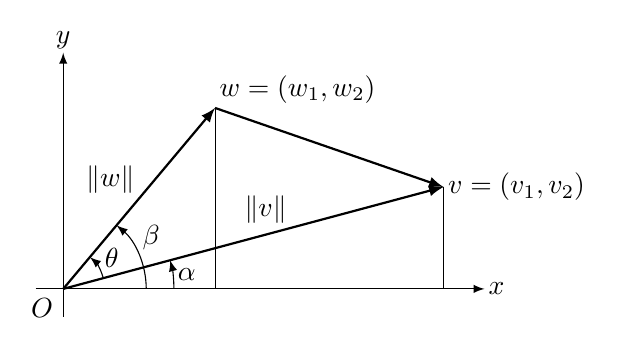
\begin{tikzpicture}[>=latex,inner sep=0.3ex]
\def\vlen{5}
\def\wlen{3}
\def\angAlpha{15}
\def\angBeta{50}
\coordinate (o) at (0,0);
\coordinate (v) at (\angAlpha:\vlen);
\coordinate (w) at (\angBeta:\wlen);
\node[below left=0.5ex] (O) at (o) {$O$};
\draw[->] (0,-1em) -- (0,\wlen) node[above] {$y$};
\draw[->] (-1em,0) -- (\vlen,0) -- +(1em,0) node[right] {$x$};
\draw[->,thick] (o) -- (v) node[right] {$v = (v_1,v_2)$} node[pos=0.6,above left] {$\lVert v \rVert$};
\draw[->,thick] (o) -- (w) node[above right] {$w = (w_1,w_2)$} node[midway,above left] {$\lVert w \rVert$};
\draw[->,thick] (w) -- (v);
\draw[very thin] (w |- o) -- (w) (v |- o) -- (v);
\def\radius{4em}
\draw[->,thin] (2:\radius) node[above right] {$\alpha$} (\radius,0) arc (0:\angAlpha:\radius);
\def\radius{3em}
\draw[->,thin] (25:\radius) node[above right] {$\beta$} (\radius,0) arc (0:\angBeta:\radius);
\def\radius{1.5em}
\draw[->,thin] (25:\radius) node[above right] {$\theta$} (\angAlpha:\radius) arc (\angAlpha:\angBeta:\radius);
\end{tikzpicture}
\end{document}